\documentclass[a4paper]{report}
\usepackage[english]{babel}
\usepackage{a4wide}
\usepackage{hyperref}
\usepackage{graphicx}
\usepackage{amsmath}
%\usepackage{amssymb}
\usepackage{tabularx}
\usepackage{longtable}
%\usepackage[utf8]{inputenc}
\usepackage{listings}
% \usepackage{booktabs}.
\usepackage{array}
\usepackage[export]{adjustbox}
\usepackage{graphicx}
\usepackage{tabularray}

% \input{includes/extra/lst_define_languages}


\title{Journal}
\author{Gilbert Fran\c cois Duivesteijn}

\begin{document}

\newcommand\ooa{1.00}
\newcommand\oob{0.495}
\newcommand\ooc{0.325}
\newcommand\ood{0.24}
\newcommand\ooe{0.195}
\newcommand\oof{0.145}
\newcommand\oog{0.137}
\newcommand\ooh{0.120}
%
% \newcommand\ts{\noindent\texttt{#1}}[1]
% \newcommand\day{\section*{#1}}[1]
\newcolumntype{Y}{>{\raggedright\arraybackslash}X}
\maketitle


\section*{11.03.2026}

\subsection*{Focus}
Main goals for the day.

\subsection*{Activities}
\begin{enumerate}
	\item \label{20260311:a1} Resnet18 with freeze blocks [0], input size $960 \times 544$
\end{enumerate}

\subsection*{Setup / Context}
Anything needed to understand the work.

\subsection*{Results}
\begin{itemize}
	\item Results of activity \ref{20260311:a1} seem worse than models from Resnet 10, which is unexpected. The $mAP$ was significantly lower, highest measured on the validation set around $0.75$.
\end{itemize}

\begin{figure}[hbt]
	\begin{center}
		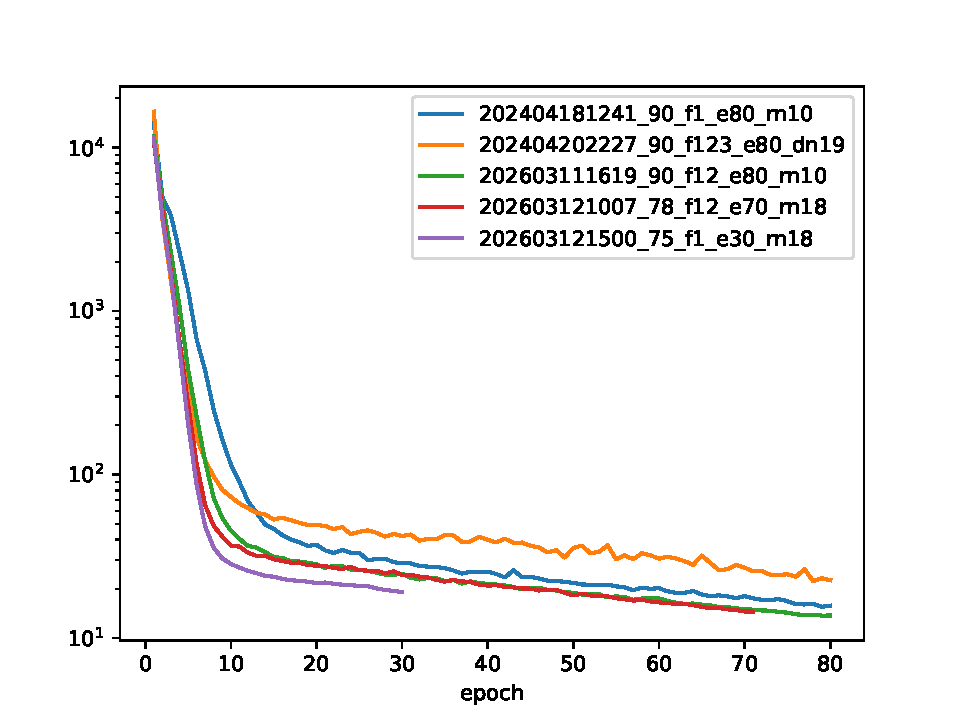
\includegraphics[width=\oob\textwidth]{assets/20260312/plot_loss_train.pdf}
		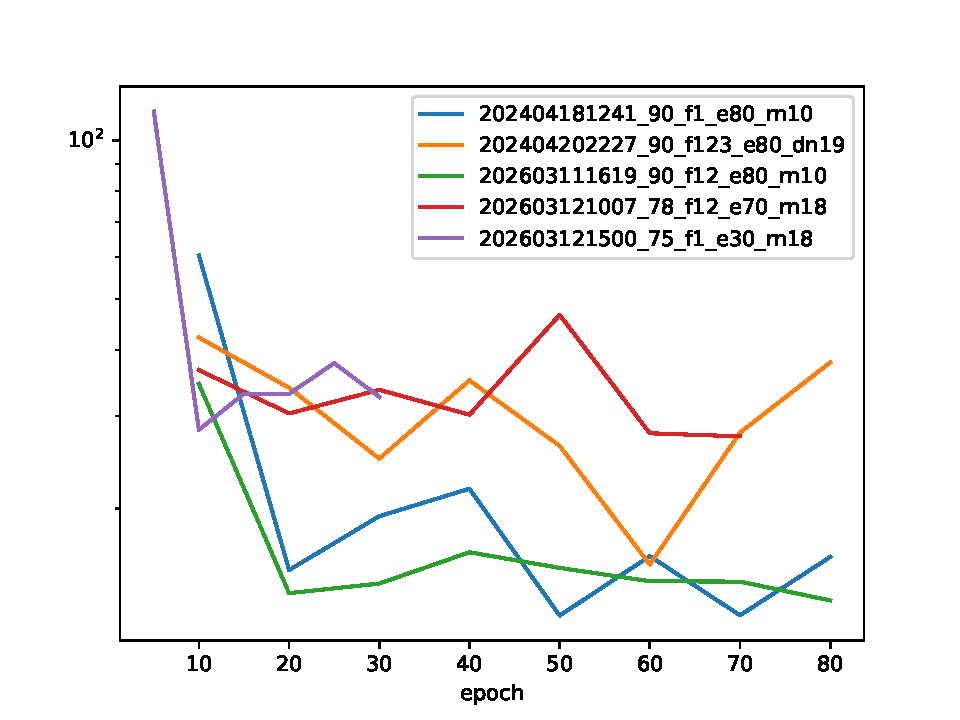
\includegraphics[width=\oob\textwidth]{assets/20260312/plot_loss_validation.pdf}
		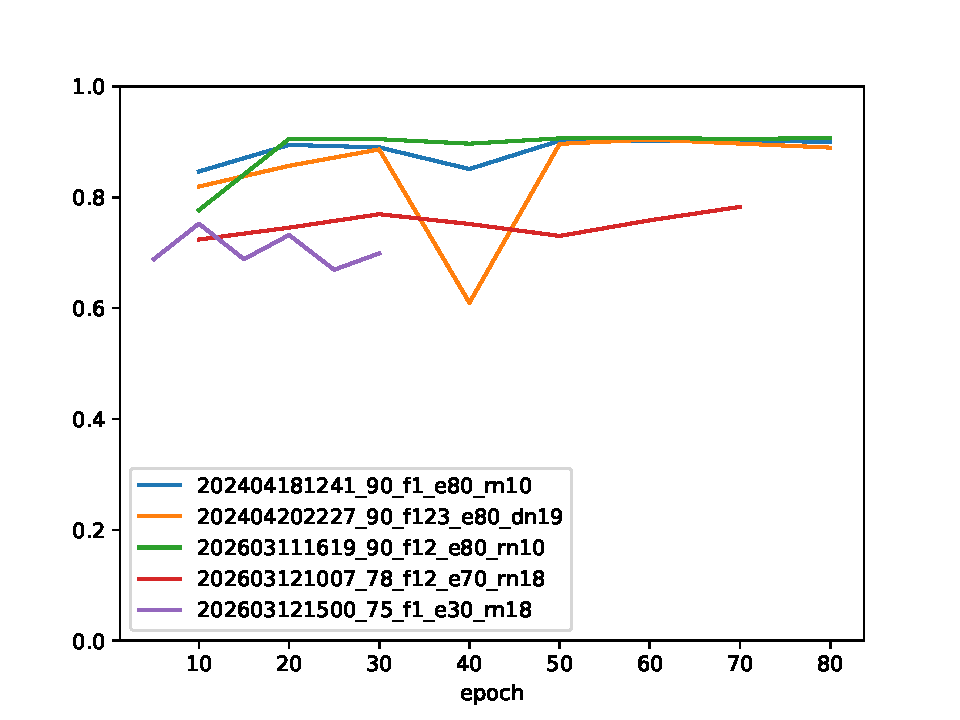
\includegraphics[width=\oob\textwidth]{assets/20260312/plot_mAP.pdf}
		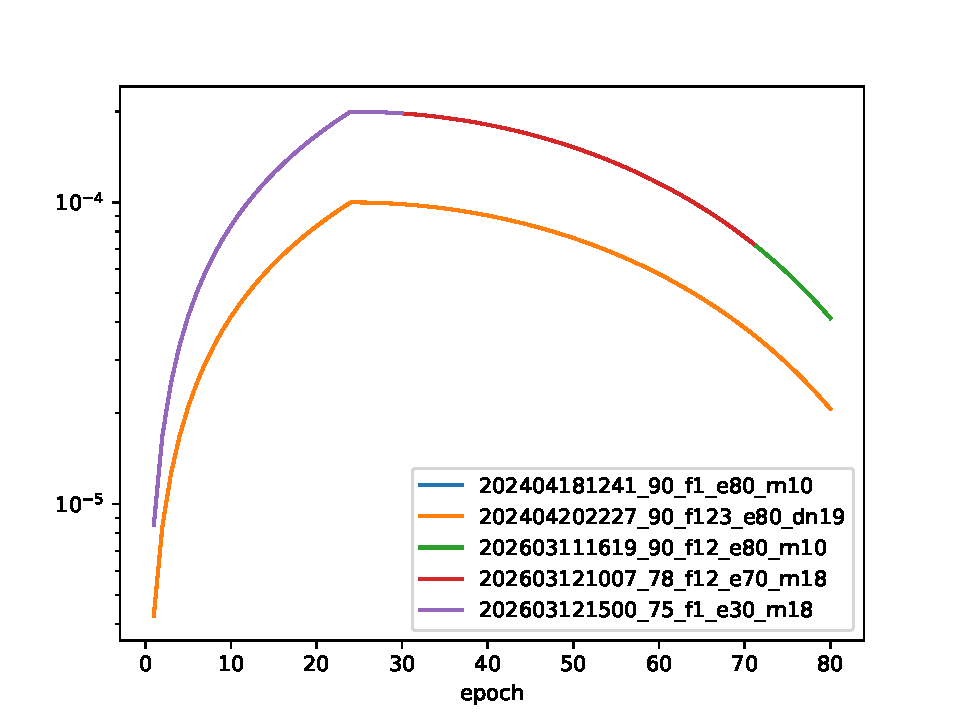
\includegraphics[width=\oob\textwidth]{assets/20260312/plot_lr.pdf}
	\end{center}
	\caption{Training metrics: $L_{train}$, $L_{val}$, mean average precision $mAP$ and learning rate}
	\label{20240105-1}
\end{figure}






\subsection*{Thoughts}
Reflections, ideas, frustrations, insights.

\subsection*{Next Steps}
Immediate follow-ups.

\subsection*{Loose Notes}
Small reminders, side ideas, references.






\section*{12.03.2026}


\subsection*{Focus}
Improving person counter for Safos.

\subsection*{Activities}
\begin{itemize}
	\item Finished training model 20260310
	\item Start training resnet18, freeze blocks 0, 1, lowered max learning rate from $1\cdot 10^{-4}$ to $5\cdot 10^{-5}$
	\item Processing corrected annotations and creating improved dataset. New training dataset 202603121637.
\end{itemize}

% \subsection*{Setup / Context}
% Anything needed to understand the work.

\subsection*{Results}
Training dataset 202603121637, number of samples 36799, containing datasets:
\begin{verbatim}
	/gilbert_lab/s3/data/person_topview/office
	/gilbert_lab/s3/data/person_topview/office_synth_exposure
	/gilbert_lab/s3/data/person_topview/onsite-2023-11-30_synth_exposure
	/gilbert_lab/s3/data/person_topview/onsite-2024-02-21
	/gilbert_lab/s3/data/person_topview/onsite-2024-03-13
	/gilbert_lab/s3/data/person_topview/onsite-2024-04-17-01
	/gilbert_lab/s3/data/person_topview/onsite-2024-04-17-02
	/gilbert_lab/s3/data/person_topview/onsite-2024-04-17-03
	/gilbert_lab/s3/data/person_topview/set3
	/gilbert_lab/s3/data/person_topview/set4
	/gilbert_lab/s3/data/person_topview/set6
	/gilbert_lab/s3/data/person_topview/set9
	/gilbert_lab/s3/data/person_topview/set_hda_cam2
	/mnt/data-gilbert-2/axpo-onsite-20251128/export
	/mnt/data-gilbert-2/swica-onsite-20240611/export
\end{verbatim}
\begin{figure}
	\begin{center}
		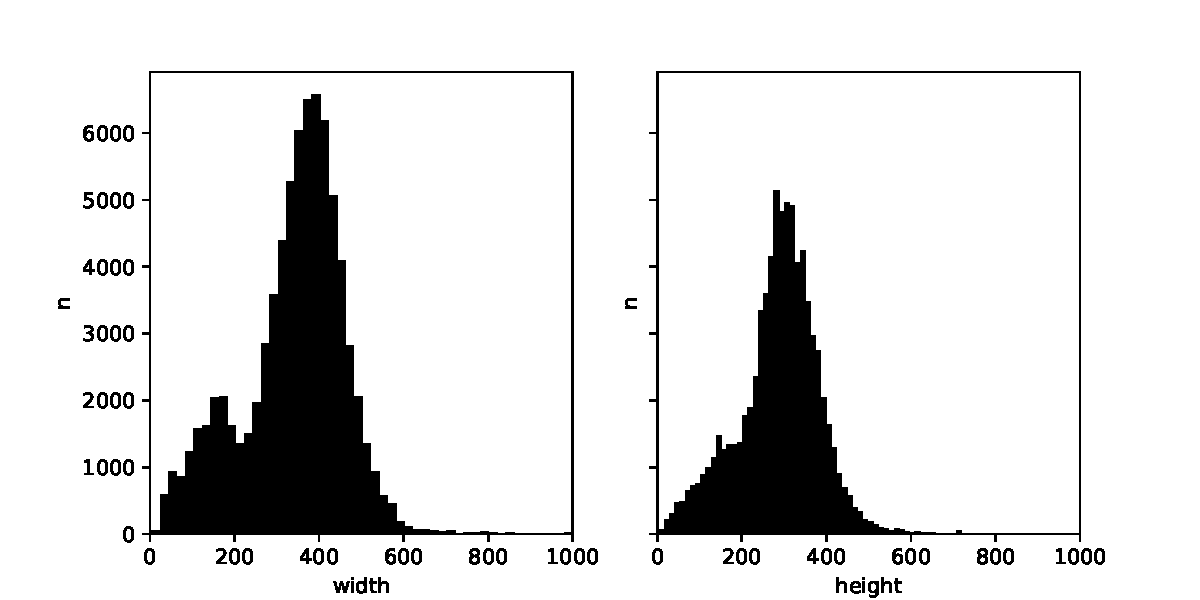
\includegraphics[width=\oob\textwidth]{assets/20260312/plot_bboxes_dist.pdf}
	\end{center}
	\caption{Distribution of bounding box sizes in the dataset 202603121637. Note that the bounding boxes are larger than usual in this type of detection models.}
\end{figure}

% \subsection*{Thoughts}
% Reflections, ideas, frustrations, insights.
%
\subsection*{Next Steps}
Immediate follow-ups.

\subsection*{Loose Notes}
Small reminders, side ideas, references.
Lorum ipsum


\section*{13.03.2026}

\subsection*{Focus}
Main goals for the day.

\subsection*{Activities}
\begin{itemize}
	\item Visit Axpo to install an updated model and observe results.
	\item Process results from Axpo in the office.
	\item Investigate input data shape for AX Facedetector v3, to see if it can be used for the person counter.
\end{itemize}

\subsection*{Results}
\begin{table}
\begin{tblr}{
  width = \textwidth,
  colspec = {Q[l,t,0.33\textwidth] Q[l,t,0.60\textwidth]},
  vlines, hlines,
  vertical = t % Ensures all cells in the row anchor at the top
}
Frame & Remark \\
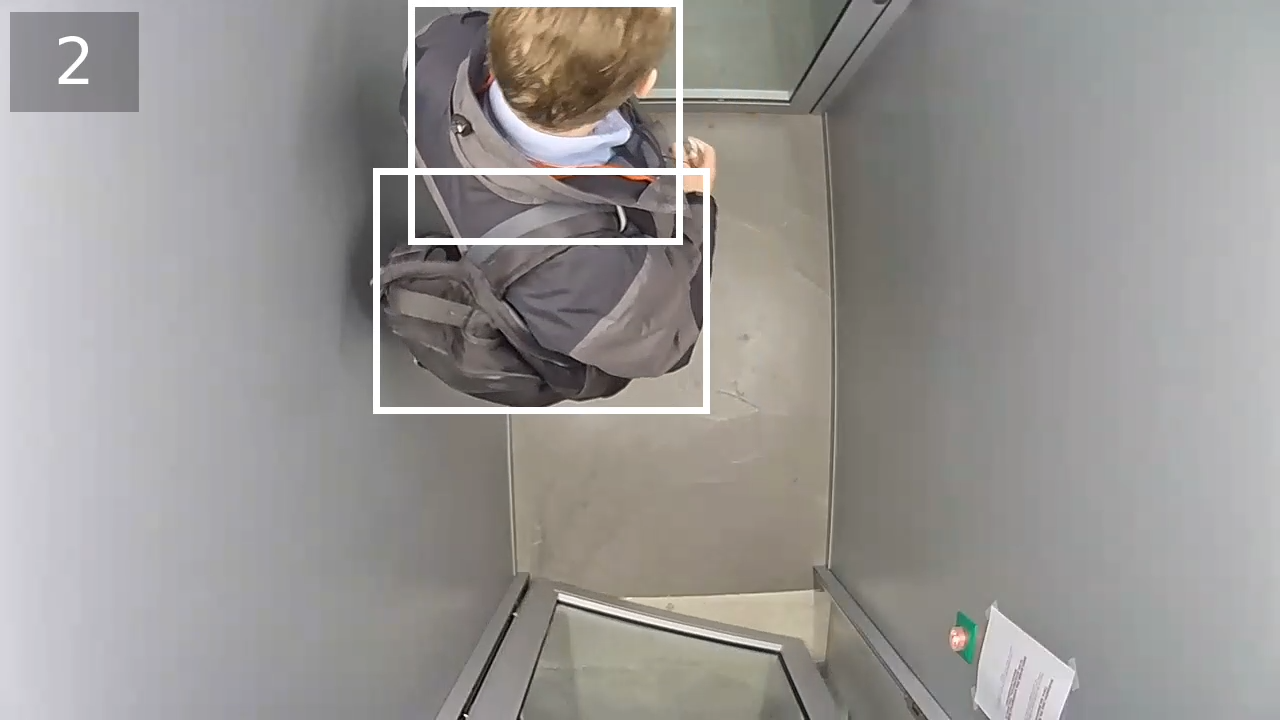
\includegraphics[width=\linewidth, valign=t]{assets/20260313/20260313074217568404737 00:06:05.png} 
& 
Observing 2 bounding boxes... \\
\end{tblr}
\caption{Frames from recording on location.}
\end{table}



%
% \subsection*{Thoughts}
% Reflections, ideas, frustrations, insights.
%
% \subsection*{Next Steps}
% Immediate follow-ups.
%
% \subsection*{Loose Notes}
% Small reminders, side ideas, references.







% \clearpage
% \bibliographystyle{ieeetr}
% \bibliography{includes/extra/references.bib}

% \section*{2026-03-12 --- Daily Lab Journal}
%
% \subsection*{Focus}
% Main goals for the day.
%
% \subsection*{Activities}
% Chronological log of what you did.
%
% \subsection*{Setup / Context}
% Anything needed to understand the work.
%
% \subsection*{Results}
% What changed, what was produced, what was decided.
%
% \subsection*{Thoughts}
% Reflections, ideas, frustrations, insights.
%
% \subsection*{Next Steps}
% Immediate follow-ups.
%
% \subsection*{Loose Notes}
% Small reminders, side ideas, references.

\end{document}
